\documentclass{standalone}
\usepackage{tikz}
\usetikzlibrary{patterns, positioning}


\begin{document}
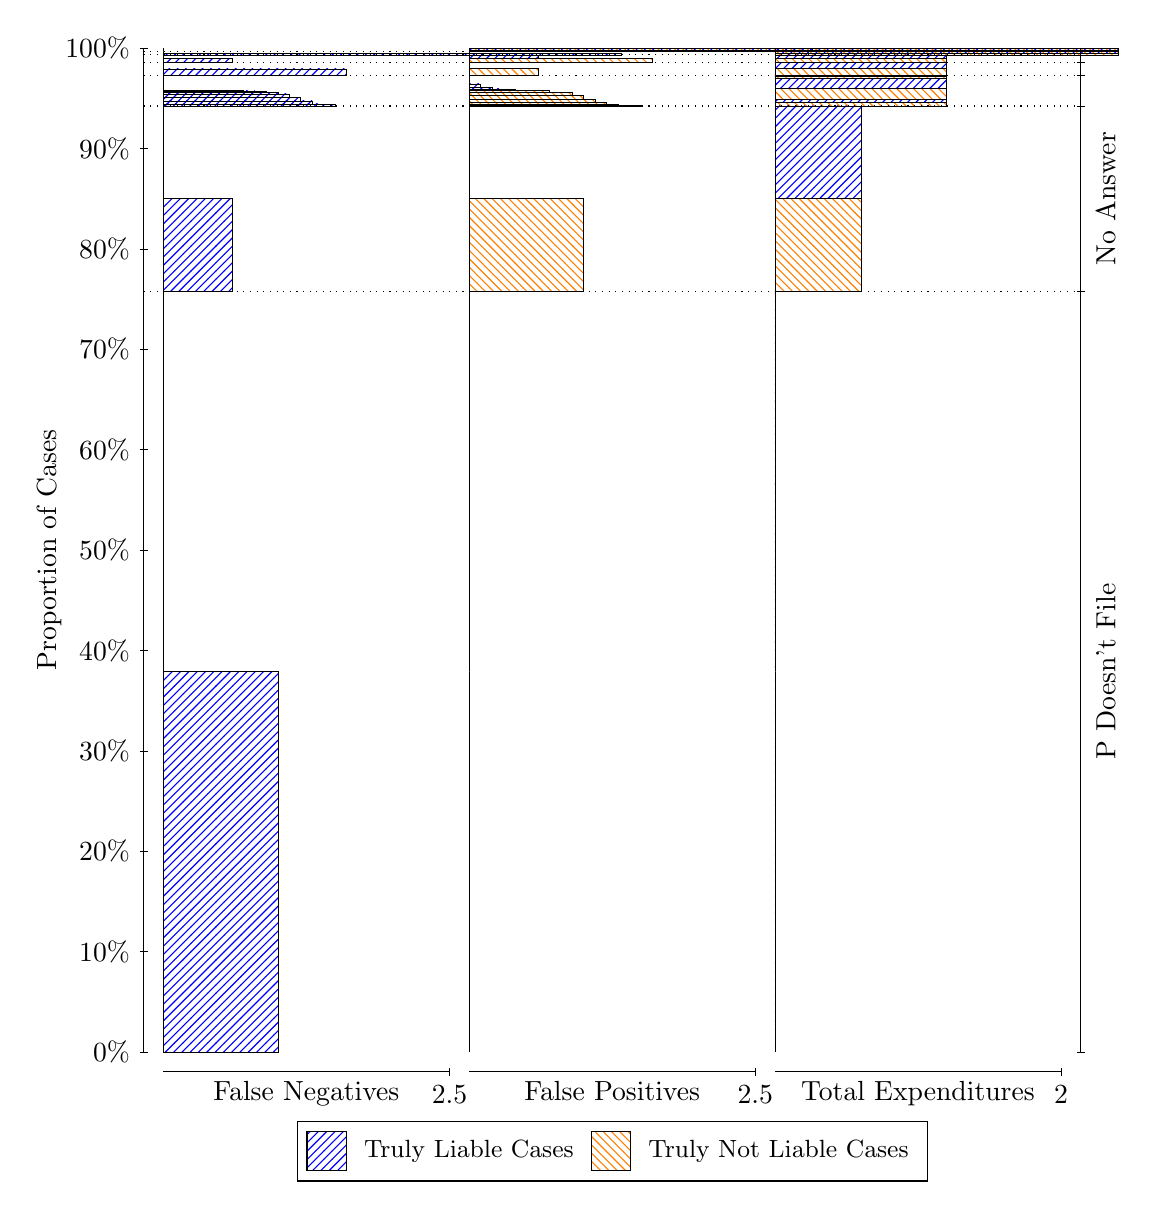
\begin{tikzpicture}
\draw[black, very thin] (1.5,1.75) -- (1.5,14.5);
\node[rotate=90, text=black, anchor=center] at (0.3, 8.125) {Proportion of Cases};
\draw[black, very thin] (1.45,1.75) -- (1.55,1.75);
\node[text=black, anchor=east] at (1.45, 1.75) {0\%};
\draw[black, very thin] (1.45,3.025) -- (1.55,3.025);
\node[text=black, anchor=east] at (1.45, 3.025) {10\%};
\draw[black, very thin] (1.45,4.3) -- (1.55,4.3);
\node[text=black, anchor=east] at (1.45, 4.3) {20\%};
\draw[black, very thin] (1.45,5.575) -- (1.55,5.575);
\node[text=black, anchor=east] at (1.45, 5.575) {30\%};
\draw[black, very thin] (1.45,6.85) -- (1.55,6.85);
\node[text=black, anchor=east] at (1.45, 6.85) {40\%};
\draw[black, very thin] (1.45,8.125) -- (1.55,8.125);
\node[text=black, anchor=east] at (1.45, 8.125) {50\%};
\draw[black, very thin] (1.45,9.4) -- (1.55,9.4);
\node[text=black, anchor=east] at (1.45, 9.4) {60\%};
\draw[black, very thin] (1.45,10.675) -- (1.55,10.675);
\node[text=black, anchor=east] at (1.45, 10.675) {70\%};
\draw[black, very thin] (1.45,11.95) -- (1.55,11.95);
\node[text=black, anchor=east] at (1.45, 11.95) {80\%};
\draw[black, very thin] (1.45,13.225) -- (1.55,13.225);
\node[text=black, anchor=east] at (1.45, 13.225) {90\%};
\draw[black, very thin] (1.45,14.5) -- (1.55,14.5);
\node[text=black, anchor=east] at (1.45, 14.5) {100\%};

\draw[black, very thin] (13.4,1.75) -- (13.4,14.5);
\draw[black, very thin] (13.35,1.75) -- (13.45,1.75);
\node[anchor=west] at (13.35, 1.75) {};
\draw[black, very thin] (13.35,11.413) -- (13.45,11.413);
\node[anchor=west] at (13.35, 11.413) {};
\draw[black, very thin] (13.35,13.764) -- (13.45,13.764);
\node[anchor=west] at (13.35, 13.764) {};
\draw[black, very thin] (13.35,14.155) -- (13.45,14.155);
\node[anchor=west] at (13.35, 14.155) {};
\draw[black, very thin] (13.35,14.317) -- (13.45,14.317);
\node[anchor=west] at (13.35, 14.317) {};
\draw[black, very thin] (13.35,14.414) -- (13.45,14.414);
\node[anchor=west] at (13.35, 14.414) {};
\draw[black, very thin] (13.35,14.457) -- (13.45,14.457);
\node[anchor=west] at (13.35, 14.457) {};
\draw[black, very thin] (13.35,14.5) -- (13.45,14.5);
\node[anchor=west] at (13.35, 14.5) {};

\draw[black, very thin, pattern color=blue, pattern=north east lines] (1.75,1.75) rectangle (3.2033,6.5814);
\draw[black, very thin, pattern color=orange, pattern=north west lines] (1.75,6.5814) rectangle (1.75,11.413);
\draw[black, very thin, pattern color=blue, pattern=north east lines] (1.75,11.413) rectangle (2.622,12.588);
\draw[black, very thin, pattern color=orange, pattern=north west lines] (1.75,12.588) rectangle (1.75,13.764);
\draw[black, very thin, pattern color=blue, pattern=north east lines] (1.75,13.764) rectangle (3.93,13.781);
\draw[black, very thin, pattern color=blue, pattern=north east lines] (1.75,13.781) rectangle (3.7847,13.79);
\draw[black, very thin, pattern color=blue, pattern=north east lines] (1.75,13.79) rectangle (3.6393,13.828);
\draw[black, very thin, pattern color=blue, pattern=north east lines] (1.75,13.828) rectangle (3.494,13.875);
\draw[black, very thin, pattern color=blue, pattern=north east lines] (1.75,13.875) rectangle (3.3487,13.918);
\draw[black, very thin, pattern color=blue, pattern=north east lines] (1.75,13.918) rectangle (3.2033,13.936);
\draw[black, very thin, pattern color=blue, pattern=north east lines] (1.75,13.936) rectangle (3.058,13.949);
\draw[black, very thin, pattern color=blue, pattern=north east lines] (1.75,13.949) rectangle (2.9127,13.955);
\draw[black, very thin, pattern color=blue, pattern=north east lines] (1.75,13.955) rectangle (2.7673,13.96);
\draw[black, very thin, pattern color=orange, pattern=north west lines] (1.75,13.96) rectangle (1.75,14.155);
\draw[black, very thin, pattern color=blue, pattern=north east lines] (1.75,14.155) rectangle (4.0753,14.236);
\draw[black, very thin, pattern color=orange, pattern=north west lines] (1.75,14.236) rectangle (1.75,14.317);
\draw[black, very thin, pattern color=blue, pattern=north east lines] (1.75,14.317) rectangle (2.622,14.366);
\draw[black, very thin, pattern color=orange, pattern=north west lines] (1.75,14.366) rectangle (1.75,14.414);
\draw[black, very thin, pattern color=blue, pattern=north east lines] (1.75,14.414) rectangle (7.5633,14.433);
\draw[black, very thin, pattern color=orange, pattern=north west lines] (1.75,14.433) rectangle (1.75,14.457);
\draw[black, very thin, pattern color=orange, pattern=north west lines] (1.75,14.457) rectangle (1.75,14.477);
\draw[black, very thin, pattern color=blue, pattern=north east lines] (1.75,14.477) rectangle (1.75,14.5);
\draw[black, very thin, pattern color=orange, pattern=north west lines] (5.6333,1.75) rectangle (5.6333,6.5814);
\draw[black, very thin, pattern color=blue, pattern=north east lines] (5.6333,6.5814) rectangle (5.6333,11.413);
\draw[black, very thin, pattern color=orange, pattern=north west lines] (5.6333,11.413) rectangle (7.0867,12.589);
\draw[black, very thin, pattern color=blue, pattern=north east lines] (5.6333,12.589) rectangle (5.6333,13.764);
\draw[black, very thin, pattern color=orange, pattern=north west lines] (5.6333,13.764) rectangle (7.8133,13.769);
\draw[black, very thin, pattern color=orange, pattern=north west lines] (5.6333,13.769) rectangle (7.668,13.775);
\draw[black, very thin, pattern color=orange, pattern=north west lines] (5.6333,13.775) rectangle (7.5227,13.788);
\draw[black, very thin, pattern color=orange, pattern=north west lines] (5.6333,13.788) rectangle (7.3773,13.805);
\draw[black, very thin, pattern color=orange, pattern=north west lines] (5.6333,13.805) rectangle (7.232,13.848);
\draw[black, very thin, pattern color=orange, pattern=north west lines] (5.6333,13.848) rectangle (7.0867,13.894);
\draw[black, very thin, pattern color=orange, pattern=north west lines] (5.6333,13.894) rectangle (6.9413,13.932);
\draw[black, very thin, pattern color=orange, pattern=north west lines] (5.6333,13.932) rectangle (6.796,13.94);
\draw[black, very thin, pattern color=orange, pattern=north west lines] (5.6333,13.94) rectangle (6.6507,13.958);
\draw[black, very thin, pattern color=blue, pattern=north east lines] (5.6333,13.958) rectangle (6.36,13.964);
\draw[black, very thin, pattern color=blue, pattern=north east lines] (5.6333,13.964) rectangle (6.2147,13.97);
\draw[black, very thin, pattern color=blue, pattern=north east lines] (5.6333,13.97) rectangle (6.0693,13.982);
\draw[black, very thin, pattern color=blue, pattern=north east lines] (5.6333,13.982) rectangle (5.924,14);
\draw[black, very thin, pattern color=blue, pattern=north east lines] (5.6333,14) rectangle (5.7787,14.044);
\draw[black, very thin, pattern color=blue, pattern=north east lines] (5.6333,14.044) rectangle (5.6333,14.155);
\draw[black, very thin, pattern color=orange, pattern=north west lines] (5.6333,14.155) rectangle (6.5053,14.237);
\draw[black, very thin, pattern color=blue, pattern=north east lines] (5.6333,14.237) rectangle (5.6333,14.317);
\draw[black, very thin, pattern color=orange, pattern=north west lines] (5.6333,14.317) rectangle (7.9587,14.365);
\draw[black, very thin, pattern color=blue, pattern=north east lines] (5.6333,14.365) rectangle (6.5053,14.414);
\draw[black, very thin, pattern color=orange, pattern=north west lines] (5.6333,14.414) rectangle (5.6333,14.437);
\draw[black, very thin, pattern color=blue, pattern=north east lines] (5.6333,14.437) rectangle (5.6333,14.457);
\draw[black, very thin, pattern color=orange, pattern=north west lines] (5.6333,14.457) rectangle (11.447,14.477);
\draw[black, very thin, pattern color=blue, pattern=north east lines] (5.6333,14.477) rectangle (9.9933,14.5);
\draw[black, very thin, pattern color=orange, pattern=north west lines] (9.5167,1.75) rectangle (9.5167,6.5814);
\draw[black, very thin, pattern color=blue, pattern=north east lines] (9.5167,6.5814) rectangle (9.5167,11.413);
\draw[black, very thin, pattern color=orange, pattern=north west lines] (9.5167,11.413) rectangle (10.607,12.589);
\draw[black, very thin, pattern color=blue, pattern=north east lines] (9.5167,12.589) rectangle (10.607,13.764);
\draw[black, very thin, pattern color=orange, pattern=north west lines] (9.5167,13.764) rectangle (11.697,13.806);
\draw[black, very thin, pattern color=blue, pattern=north east lines] (9.5167,13.806) rectangle (11.697,13.85);
\draw[black, very thin, pattern color=orange, pattern=north west lines] (9.5167,13.85) rectangle (11.697,13.983);
\draw[black, very thin, pattern color=blue, pattern=north east lines] (9.5167,13.983) rectangle (11.697,14.118);
\draw[black, very thin, pattern color=orange, pattern=north west lines] (9.5167,14.118) rectangle (11.697,14.137);
\draw[black, very thin, pattern color=blue, pattern=north east lines] (9.5167,14.137) rectangle (11.697,14.155);
\draw[black, very thin, pattern color=orange, pattern=north west lines] (9.5167,14.155) rectangle (11.697,14.237);
\draw[black, very thin, pattern color=blue, pattern=north east lines] (9.5167,14.237) rectangle (11.697,14.317);
\draw[black, very thin, pattern color=orange, pattern=north west lines] (9.5167,14.317) rectangle (11.697,14.365);
\draw[black, very thin, pattern color=blue, pattern=north east lines] (9.5167,14.365) rectangle (11.697,14.414);
\draw[black, very thin, pattern color=orange, pattern=north west lines] (9.5167,14.414) rectangle (13.877,14.437);
\draw[black, very thin, pattern color=blue, pattern=north east lines] (9.5167,14.437) rectangle (13.877,14.457);
\draw[black, very thin, pattern color=orange, pattern=north west lines] (9.5167,14.457) rectangle (13.877,14.477);
\draw[black, very thin, pattern color=blue, pattern=north east lines] (9.5167,14.477) rectangle (13.877,14.5);
\draw[black, dotted] (1.5,11.413) -- (13.4,11.413);
\draw[black, dotted] (1.5,13.764) -- (13.4,13.764);
\draw[black, dotted] (1.5,14.155) -- (13.4,14.155);
\draw[black, dotted] (1.5,14.317) -- (13.4,14.317);
\draw[black, dotted] (1.5,14.414) -- (13.4,14.414);
\draw[black, dotted] (1.5,14.457) -- (13.4,14.457);
\draw[black, very thin] (1.75,1.5) -- (5.3833,1.5);
\node[text=black, anchor=north] at (3.5667, 1.5) {False Negatives};
\draw[black, very thin] (5.3833,1.45) -- (5.3833,1.55);
\node[text=black, anchor=north] at (5.3833, 1.45) {2.5};

\draw[black, very thin] (5.6333,1.5) -- (9.2667,1.5);
\node[text=black, anchor=north] at (7.45, 1.5) {False Positives};
\draw[black, very thin] (9.2667,1.45) -- (9.2667,1.55);
\node[text=black, anchor=north] at (9.2667, 1.45) {2.5};

\draw[black, very thin] (9.5167,1.5) -- (13.15,1.5);
\node[text=black, anchor=north] at (11.333, 1.5) {Total Expenditures};
\draw[black, very thin] (13.15,1.45) -- (13.15,1.55);
\node[text=black, anchor=north] at (13.15, 1.45) {2};

\node[text=black, centered, rotate=90] at (13.72, 6.5814) {P Doesn't File};
\node[text=black, centered, rotate=90] at (13.72, 12.588) {No Answer};






\draw (7.449999999999999,1.5) node[draw=none] (baseCoordinate) {};
\begin{scope}[align=center]
        \matrix[scale=0.5, draw=black, below=0.5cm of baseCoordinate, nodes={draw}, column sep=0.1cm]{
            \node[rectangle, draw, minimum width=0.5cm, minimum height=0.5cm, pattern color=blue, pattern=north east lines] {}; &
            \node[draw=none, font=\small, text=black] (B) {Truly Liable Cases}; &
            \node[rectangle, draw, minimum width=0.5cm, minimum height=0.5cm, pattern color=orange, pattern=north west lines] {}; &
            \node[draw=none, font=\small, text=black] (B) {Truly Not Liable Cases}; \\
            };
\end{scope}

\end{tikzpicture}
\end{document}